%File: formatting-instruction.tex
\documentclass[letterpaper]{article}
\usepackage{caption}
%\DeclareCaptionType{copyrightbox}
%\graphicspath{{./figures/}}
\usepackage{subcaption}
\usepackage{url}
\usepackage{graphicx}
%\usepackage{epstopdf}
\usepackage{multirow}
\usepackage{amsmath, amsfonts, amssymb}
\graphicspath{{./figures/}}
\usepackage{color}
%package for proper unicode rendering
\usepackage[utf8]{inputenc}
\usepackage{url}
\usepackage{aaai}
\usepackage{times}
\usepackage{helvet}
\usepackage{courier}

\setlength{\titlebox}{2.8in}
\inputencoding{utf8}

\frenchspacing
\setlength{\pdfpagewidth}{8.5in}
\setlength{\pdfpageheight}{11in}
\pdfinfo{
/Title (Insert Your Title Here)
/Author (Put All Your Authors Here, Separated by Commas)}
\setcounter{secnumdepth}{0}  
 \begin{document}
\newcommand{\narenc}[1]{[{\color{red} Naren writes: \it #1}]}
\newcommand{\sathappanc}[1]{[{\color{blue} Sathappan writes: \it #1}]}
\newcommand{\then}{\Rightarrow}
\newcommand{\softor}{\operatornamewithlimits{\tilde{\vee}}}
\newcommand{\softand}{\operatornamewithlimits{\tilde{\wedge}}}
\newcommand{\softthen}{\operatornamewithlimits{\tilde{\then}}}
\newcommand{\softneg}{\operatornamewithlimits{\tilde{\neg}}}
%\title{Forecasting Protests \\by Detecting Future Time Mentions \\in News and Social Media}
\title{Planned Protest Modeling in News and Social Media}
\author{
% 1st. author
Sathappan Muthiah\\
Virginia Tech\\
Arlington, VA 22203\\
sathap1@cs.vt.edu
% 2nd. author
\And
Bert Huang\\
       University of Maryland\\
       College Park, MD 20742\\
       bert@cs.umd.edu
%% 3rd. author
       \And
Jaime Arredondo\\
       University of California\\
       San Diego, CA 92093\\
       jarredon@ucsd.edu
\AND 
% use '\and' if you need 'another row' of author names
%% 4th. author
David Mares\\
       University of California\\
       San Diego, CA 92093\\
       dmares@ucsd.edu
%% 5th. author
       \And
Lise Getoor\\
       University of California\\
       Santa Cruz, CA 95064\\
       getoor@soe.ucsc.edu
%% 6th. author
       \And
Graham Katz\\
       CACI Inc.\\
       Lanham, MD 20706\\
       ekatz@caci.com
%\AND
       \And
%% 7th. author
Naren Ramakrishnan\\
       Virginia Tech\\
       Arlington, VA 22203\\
       naren@cs.vt.edu
}
\maketitle
\begin{abstract}
\begin{quote}
Civil unrest (protests, strikes, and ``occupy'' events) is a common occurrence in both democracies and authoritarian regimes. The study of civil unrest is a key topic for political scientists as it helps capture an important mechanism by which citizenry express themselves. In countries where civil unrest is lawful, qualitative analysis has revealed that more than 75\% of the protests are planned, organized, and/or announced in advance; therefore detecting future time mentions in relevant news and social media is a direct way to develop a protest forecasting system. We develop such a system in this paper, using a combination of key phrase learning to identify what to look for, probabilistic soft logic to reason about location occurrences in extracted results, and time normalization to resolve future tense mentions. We illustrate the application of our system to 10 countries in Latin America, viz. Argentina, Brazil, Chile, Colombia, Ecuador, El Salvador, Mexico, Paraguay, Uruguay, and Venezuela. Results demonstrate our successes in capturing significant societal unrest in these countries with an average lead time of 4.08 days. We also study the selective superiorities of news media versus social media (Twitter, Facebook) to identify relevant tradeoffs.
\end{quote}
\end{abstract}
%\section{Introduction}
\label{intro}
Civil unrest (protests, strikes, and ``occupy'' events) is a common happening in both democracies
and authoritarian regimes.
Although we typically associate civil unrest with disruptions and instability, for a social scientist
civil unrest reflects the democratic process by 
which citizenry communicate their views and preferences to those in authority. 
The advent of social
media has afforded citizenry new mechanisms for organization and mobilization, and online news sources
and social networking sites like Facebook and Twitter
can provide a window into civil unrest happenings in a particular country.

\vspace{-0.5em}
\subsubsection{Why study and forecast protests?}
Our region of interest is Latin America and protest is an important
topic of study here, as many countries here are democracies struggling
to consolidate themselves. The combination of weak channels of
communication between citizen and government, and a citizenry that still
has not grasped the desirability of elections as the means to affect
politics means that public protest will be an especially attractive
option. To illustrate the power of protest in Latin America we need only
recall that between 1985 and 2011, 17 presidents resigned or were
impeached under pressure from demonstrations, usually violent, in the
streets. Protests have also resulted in the rollback of price increases
for public services, such as during the ‘Brazilian Spring’ of June 2013.

Forecasting protests is an important capability in many domains.
For the tourism industry, forecasting protests can
support the issuance of travel warnings. For law enforcement,
forecasting protests can aid in preparedness. For the social scientist,
protests forecasts will provide insight into how citizens express themselves.
For the government, a protest forecasting system can help prioritize
citizen grievances. Finally, protests can have a debilitating effect on
multiple industries (esp. those that rely on worldwide supply chain management)
and thus a protest forecasting system can aid in planning and design
of alternative travel and shipping routes.

\vspace{-0.5em}
\subsubsection{Planned protests}
Our basic hypothesis is that protests that are larger will be more
disruptive and communicate support for its cause better than smaller
protests.  Mobilizing large numbers of people is more likely to occur if
a protest is organized and the time and place announced in advance.
Because protest is costly and more likely to succeed if it is large, we
should expect planned, rather than spontaneous, protests to be the norm.
Indeed, in a sample of 288 events from our study selected for
qualitative review of their antecedents, for 225 we located
communications regarding the upcoming occurrence of the event in media,
and only 49 could be classified as spontaneous (we could not determine
whether communications had or had not occurred in the remaining 14
cases).

\vspace{-0.5em}
\subsubsection{EMBERS(Early Model Based Event Recognition using
Surrogates)}
We are an industry-university partnership charged with developing an
automatic protest forecasting system for 10 countries in
Latin America. Our system, called EMBERS, has been
deployed since Nov 2012 and has been generating forecasts (called
warnings or alerts) automatically, without a human-in-the-loop. These forecasts are emailed to
a third party (MITRE) for evaluation. Analysts at MITRE organize a reference
database of protests (called the Gold Standard Report,
or GSR) by surveying newspapers for reportings of protests, and
compare our warnings against the GSR to generate a scoring report (evaluation
criteria described later).

The full EMBERS system has been described elsewhere~\cite{emberskdd}, including
the overall system architecture, data sources used for analysis, and the
various forecasting models in EMBERS. EMBERS adopts a multi-model approach,
wherein different models are leveraged for their selective superiorities
to generate a fused set of alerts. Arguably, one of the
best performing models in EMBERS is the planned protest model that detects
ongoing organizational activity and generates warnings accordingly. This paper
is the first to present this model in detail, including the 
research issues involved, and how we addressed them in EMBERS.

Capturing mentions of protest planning and organization 
is not as easy as it might appear. First, articles of interest are written in
different languages (Spanish, Portugese, French, Dutch, and English). 
Second, multiple locations are often mentioned in a given article, leading
to (natural language) ambiguity about the intended location of the event.
Significant reasoning is required to discern the correct protest location.
Finally, dates are often described in relative terms, e.g., `Sunday' and 
thus these vague references need to be resolved into absolute temporal
information. 

Our detection approach 
combines shallow linguistic analysis to identify a corpus of relevant
documents (articles, tweets) which are then subject to targeted deep semantic analysis.
Despite its simplicity, we are able to
detect indicators of event planning with surprisingly high
accuracy. Our contributions are:

\iffalse
\begin{figure}
    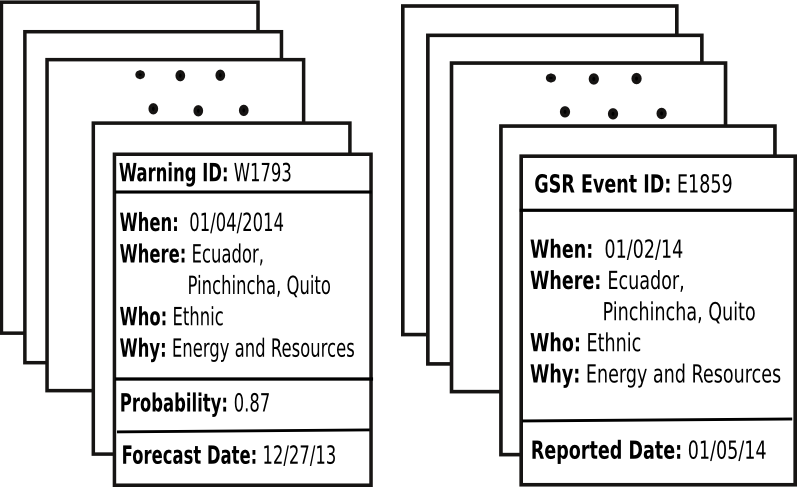
\includegraphics[width=0.5\textwidth]{alertstructure}
    \vspace{-2em}
    \caption{An example warning (left) and GSR event (right).}
    \label{fig:alertstructure}
\end{figure}
\fi

\begin{enumerate}
\item We present a protest forecasting system that couples three key
  technical ideas: key phrase learning to identify what to look for,
  probabilistic soft logic to reason about location occurrences in
  extracted results, and date normalization to resolve future tense
  mentions. We demonstrate how the integration of these ideas achieves
  objectives in precision, recall, and quality (accuracy).
\item We illustrate the application of our system to 10 countries in
  Latin America, viz. Argentina, Brazil, Chile, Colombia, Ecuador, El
  Salvador, Mexico, Paraguay, Uruguay, and Venezuela. Our system
  predicts the {\it when} of the protest as well as {\it where} of the
  protest (down to a city level granularity).  We conduct ablation
  studies to identify the relative contributions of news media (news +
  blogs) versus social media (Twitter, Facebook) to identify future
  happenings of civil unrest. Through these studies we illustrate the
  selective superiorities of different sources for specific countries.
\item Unlike many studies of retrospective forecasting of protests, our
  system has been {\bf deployed and in operation for nearly two years.}
  The end consumers of our alerts are analysts studying Latin America.
  Our results demonstrate that we are able to capture significant
  societal unrest in the above countries with an average lead time of
  4.08 days. 

\end{enumerate}

\vspace{-0.8em}
\section{Related Work}
Five categories of related work are briefly discussed here (see also
Table~\ref{comp-table}).

\begin{table*}
    \centering
    \vspace{-2em}
    \caption{Comparison of our approach against other techniques.}
    \begin{tabular}{l p{2cm} p{1.5cm} p{1.5cm} p{1.5cm} p{3cm}}%{|*{17}{c|}}
        \hline
        & Relative date resolution & Ingest multiple sources? & Reasoning about location & Learning word/phrase filters \\
        \hline
        `Future' Search Engines~\shortcite{Kawai:2010:CSE,Jatowt:2011:ECE,baeza2005searching}&\checkmark & & \\
        Time-to-Event Recognition~\shortcite{tops2013predicting,bosch2013estm}&\checkmark & & \\
        Planned Protest Detection~\shortcite{xu2014civil,compton2013detecting} & &\checkmark & &\\ 
        This paper &\checkmark &\checkmark &\checkmark&\checkmark\\  \hline
    \end{tabular}
\label{comp-table}
\end{table*}

{\bf Event detection via text extractions}
is an extensively studied topic in the literature. Document clustering
techniques are used in, e.g.,~\cite{Gabrilovich:2004:NPP} to identify
events retrospectively or as the stories arrive.  Works
like~\cite{Banko07openinformation,Chambers:2011:TIE,riloff2003learning}
focus on extraction patterns (templates) to extract information from
text.

\iffalse Ritter et al.~\cite{Ritter:2012} show that it is
possible to accurately extract a calendar of significant events from
Twitter by training a tagger for recognizing event phrases.
Sankaranarayanan et al.~\cite{Sankaranarayanan:2009:TNT} captures tweet
clusters of interest to identify late breaking News from twitter Highly
specialized applications also exist; e.g., Sakaki et
al.~\cite{Sakaki:2010:EST} mine tweets to enable prompt detection of
occurences of earthquakes.
\fi

{\bf Temporal information extraction} is another well studied topic.
The TempEval challenge~\cite{tempeval} led to a significant amount of
algorithmic development for temporal NLP.  For instance, a specification
language for temporal and event expressions in natural language text is
described in~\cite{timeml}.  Refs.~\cite{LlorensDGS12} and~\cite{tempex}
provide methods to resolve temporal expressions in text (our own work
here uses the TIMEN package~\cite{LlorensDGS12}).

{\bf Event forecasting:} 
Radinsky and Horvitz~\cite{Radinsky:2013:MWP} find event sequences from
a corpora and then use these sequences to determine if an event of
interest (e.g., a disease outbreak, or a riot) will occur sometime in
the future. This work predicts only if a potential event will happen
given a historical event sequence but does not geolocate the event to a
city-level resolution, as we do here.  Kallus~\cite{nathankallus} makes
use of event data from RecordedFuture~\cite{recordedFuture} to determine
if a  significant protest event will occur in the subsequent three days
and casts this as a classification problem.  This work only focuses on
prediction of significant events (suitably defined) and the forecast is
limited to a fixed time window of the next three days. 

{\bf Future retrieval:}
Baeza-Yates~\cite{baeza2005searching} provides one of the earliest
discussions of this topic; here future temporal information in text is
found and used to retrieve content from search queries that combine both
text and time with a simple ranking scheme.  Kawai et
al.~\cite{Kawai:2010:CSE} present a search engine (ChronoSeeker) for
searching future and past events.  RecordedFuture~\cite{recordedFuture},
introduced earlier, conducts real-time analysis of news and tweets to
identify mentions of events along with associated times. Anectodally it
is estimated that approximately (only) 5--7\% of events extracted by
RecordedFuture are about the future.  {\bf Planned protest detection:}
Two publications---Compton et al. ~\cite{compton2013detecting} and Xu et
al.~\cite{xu2014civil}---align very closely to our own work as their
emphasis is on protest forecasting.  Both works are aimed at forecasting
protests but emphasize different data sources and different
methodologies. For instance, the work in~\cite{compton2013detecting}
filters the Twitter stream for keywords of interest and searches for
future date mentions in only absolute terms, i.e., explicit mentions of
a month name and a number (date) less than 31.  Such an approach will
not be capable of extracting the more common way in which future dates
are referenced, e.g., phrases like ``tomorrow,'' ``next tuesday.'' The
work in~\cite{xu2014civil} by the same group of authors uses the Tumblr
feed with a smaller set of keywords but again is restricted to the use
of absolute time identifiers.  Furthermore, in this work, location is
restricted to membership in a whitelist of 1022 entries which would not
be able to capture the diversity of location identifiers at the city
level; the system is also unable to reason about the presence of
multiple location names.
\vspace{-0.8em}
\section{Probabilistic Soft Logic}
\label{sectionPSL}
In this section, we briefly describe probabilistic soft logic
(PSL)~\cite{kimmig2012short}, a key component of our geocoding strategy
described later.  PSL is a framework for collective probabilistic
reasoning on relational domains.  PSL represents the domain of interest
as logical atoms.  It uses first order logic rules to capture the
dependency structure of the domain, based on which it builds a joint
probabilistic model over all atoms.  Instead of hard truth values of $0$
(false) and $1$ (true), PSL uses soft truth values relaxing the truth
vlaues to the interval $[0,1]$.  The logical connectives are adapted
accordingly.  User defined \emph{predicates} are used to encode the
relationships and attributes and \emph{rules} capture the  dependencies
and constraints.  The rules can also be labeled with non-negative
weights which are used during the inference process.  The set of
predicates and weighted rules thus make up a PSL program where known
truth values of ground atoms derived from observed data and unknown
truth values for the remaining atoms are learned using the PSL
inference.

Given a set of atoms $\ell = \{\ell_1,\ldots,\ell_n\}$, an
interpretation defined as $I : \ell \rightarrow [0,1]^n$ is a mapping
from atoms to soft truth values.  PSL defines a probability distribution
over all such interpretations such that those that satisfy more ground
rules are more probable.  PSL uses the \emph{Lukasiewicz t-norm} and its
corresponding co-norm as relaxations of the logical AND and OR
respectively to determine the degree to which a ground rule is
satisfied.  Given an interpretation $\mathit{I}$, these relaxations of
logical conjunction ($\wedge$), disjunction ($\vee$), and negation
($\neg$) are
\small
\begin{align*}
\ell_1 \softand \ell_2 &= \max\{0, I(\ell_1) + I(\ell_2) - 1\},\\
\ell_1 \softor \ell_2 &= \min\{I(\ell_1) + I(\ell_2), 1\},\\
\softneg l_1 &= 1 - I(\ell_1),
\end{align*}  

\normalsize
The probability distribution over interpretations is log linear with
features defined by \emph{distances to satisfaction}, which follows the
Lukasiewicz t-norm to relax the fact that a rule $\mathit{r} \equiv
\mathit{r_{body}} \rightarrow \mathit{r_{head}} $  is satisfied if and
only if the truth value of head is at least that of the body. The rule's
distance to satisfaction measures the degree to which this condition is
violated.  \newline \small \begin{center} $\mathit{d_r}(\mathit{I}) =$
max\{0,$\mathit{I(r_{body})} - \mathit{I(r_{head})}$\} \end{center}

\normalsize PSL then induces a probability distribution over possible
interpretations $\mathit{I}$ over the given set of ground atoms
$\mathit{l} $ in the domain.  If $\mathit{R}$ is the set of all ground
rules that are instances of a rule from the system and uses only the
atoms in  $\mathit{I}$ then, the probability density function
$\mathit{f}$ over $\mathit{I}$ is defined as 
\small 
\begin{equation}
  \label{eq:contimn1} f (I) = \frac{1}{Z} \text{exp}\left(-\sum_{r\in R}
  \lambda_r (d_r(I))^p\right) \end{equation} \begin{equation}
  \label{eq:contimn2} Z = \int_{I} \text{exp} \left( -\sum_{r\in R}
\lambda_r (d_r(I))^p \right)
\end{equation}
\normalsize
where~$\lambda_r$ is the weight of the rule~$r$, $Z$ is the continuous
version of the normalization constant used in discrete Markov random
fields, and ~$p \in \{1, 2\}$ provides a choice between two different
loss functions, linear and quadratic.  The values of the atoms can be
further restricted by providing linear equality and inequality
constraints allowing one to encode functional constraints from the
domain. 

PSL enables fast inference of the most probable explanation, i.e., the
interpretation that is most likely in the PSL distribution given a
partial interpretation with grounded atoms based on observed evidence.
Because of the structure of PSL rules and their distances to
satisfaction, this inference is always solvable via a convex
optimization. Further, the structure of the probabilistic model enables
this convex optimization to be solved very quickly using the alternating
direction method of multipliers (ADMM)
\cite{boyd:ftml11,bach2012scaling,bach:uai13}. Using this approach, PSL
enables our system to easily define a rich probabilistic model and
perform inference with a lightweight computational cost. 

\vspace{-0.8em}
\section{Approach}
\begin{figure*}
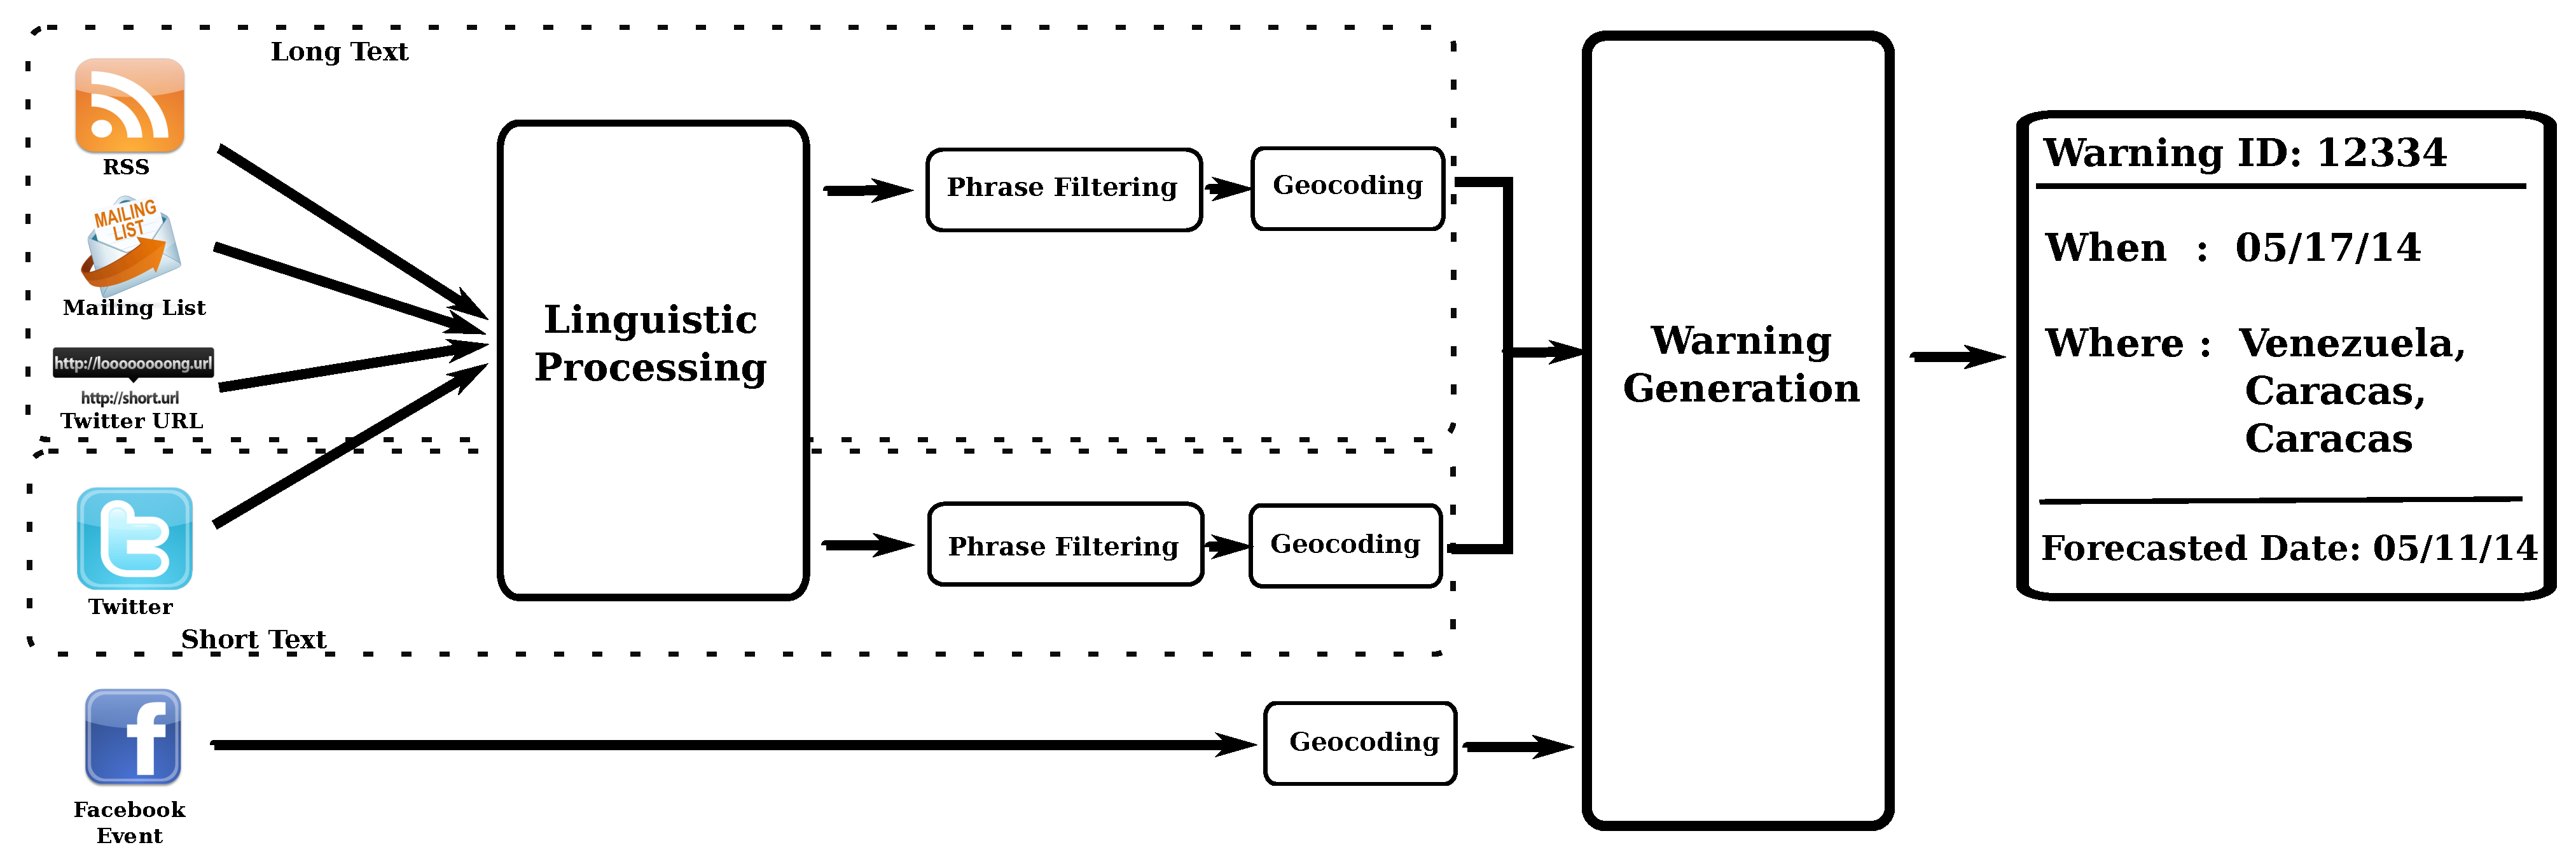
\includegraphics[width=\textwidth]{pipeline2}
\vspace{-2em}
\caption{Schematic of the planned protest detector that ingests five
different types of data sources.}
\label{flowchart}
\end{figure*}
The general approach we adopt is to identify open-source documents
that appear to indicate civil unrest event planning, extract
relevant information from identified documents and use that as the
basis for a structured warning about the planned event (see Fig.~\ref{flowchart}).

\subsection{Linguistic Preprocessing}
A wide array of textual documents---RSS feeds (news and blogs),
mailing lists, URLs referenced in tweets, the contents of the tweets themselves,
and Facebook event pages---are
subjected to shallow linguistic processing prior to analysis.  This
involves identifying the language of the document, distinguishing
the words (tokenization), normalizing words for inflection
(lemmatization), and identifying expressions referring to people,
places, dates and other entities and classifying them (named entity extraction). 
Since our region of interest is Latin America, the collection of text
harvested is inherently multilingual, with Spanish, Portugese, and English as
the dominating languages;
we use Basis Technology's Rosette Linguistics Platform (RLP) suite of
multilingual commercial tools
(\url{http://www.basistech.com/text-analytics/rosette/}) for this stage.
The output of linguistic preprocessing serves as input to subsequent deeper analysis in which 
date expressions are normalized and the geographic focus of the text identified.

Date processing is particularly crucial to the identification of
future oriented statements. We use the TIMEN~\cite{LlorensDGS12} date
normalization package to normalize and deindex expressions referring
to days in English, Spanish and Portuguese. This system makes use of
meta-data such as the day of publication, and other information about
the linguistic context of the date expression to determine for each
date expression, what day (or week, month or year) it refers to.  For
example in a tweet produced on June 10, 2014, the occurrence of the
term {\em Friday} used in a future-tense sentence {\em We'll get
  together on Friday} will be interpreted as June 13, 2014.  Each
expression identified as a date by the RLP preprocessor is normalized
in this way.

\subsection{Phrase filtering}
In order to identify relevant documents, input documents are filtered on a set of key phrases, i.e.,
the text of the document is searched for the presence of one or
more key phrases in a list of phrases which are indicative of an article's focus being
a planned civil unrest event.  
The list of key phrases indicating civil unrest planning was obtained
in a semi-automatic manner, as detailed in Section \ref{sec:phraselearning}.
Articles which do match are processed further, those that do not are ignored.

\vspace{-0.5em}
\subsubsection{Phrase matching}
Our key phrase matching is highly general and linguistically
sophisticated.  The phrases in our list are general rules for
matching, rather than literal string sequences. Typically a phrase
specification comprises: two or more word lemmas, a language
specification, and a separation threshold. This indicates that words---potentially inflected forms---in 
a given sequence potentially separated by one or more other words, should be taken to be a
match. We determined that this kind of
multi-word key phrases was more accurate than simple keywords for
extracting events of interest from the data stream.

The presence of a keyphrase is checked by searching for the presence of
individual lemmas of the keyphrase within the same sentence separated
by at most a number of words that is fewer than the separation threshold.  
This method allows for linguistically sophisticated and flexible matching, so, for example,
the keyphrase {\bf [{\em plan protest}, 4, English]} would match the sentence
{\em The students are planning a couple big protests tomorrow} in an input document.

\vspace{-0.5em}
\subsubsection{Phrase list development}
\label{sec:phraselearning}
The set of key phrases was tailored (slightly) to the genre of the
input. In particular different phrases were used to identify relevant
news articles and blogs from those used to filter Tweets.  The lists
themselves were generated semi-automatically.

Initially, a few seed phrases were obtained manually
with the help of subject matter experts.
An analysis of news reports for planned protests in the print media helped create a
minimum set of words to use in the query.  We choose four nouns from
the basic query that is used predominantly to indicate a civil unrest
in the print media - {\em demonstration, march, protest} and
{\it strike}. We translated them into Spanish and Portuguese, including
synonyms.  We then combined these with future-oriented verbs, e.g., {\em to organize}, {\em to prepare}, {\em to
plan}, and {\em to announce}. For twitter, shorter phrases were identified, and these had
a more direct call for action, e.g., {\em marchar}, {\em manhã de mobilização}, {\em
  vamos protestar}, {\em huelga}.

To generalize this set of phrases, the phrases were then parsed
using a dependency parser~\cite{freeling} and the grammatical
relationship between the core nominal focus word (e.g., {\em protest}, 
{\em manifestación}, {\em huelga}) and any accompanying
word (e.g., {\em plan}, {\em call}, {\em anunciar}) was
extracted. These grammatical relations were used as extraction
patterns as in~\cite{riloff2003learning} to learn more phrases from a
corpora of sentences extracted from the data stream of interest
(either news/blogs or tweets). This corpus consists of sentences that
contained any one of the nominal focus words and also had mentions of
a future date. The separation threshold for a phrase was also
learned, being set to the average number of words separating
the nominal focus and the accompanying word.

The set of learned phrases is then reviewed by a subject matter expert for quality contraol.  
Using this approach, we learned 112 phrases for news articles and blogs and 156 for tweets.  
This phrase learning process is illustrated in Fig.~\ref{fig:phraselearning}.

\begin{figure}
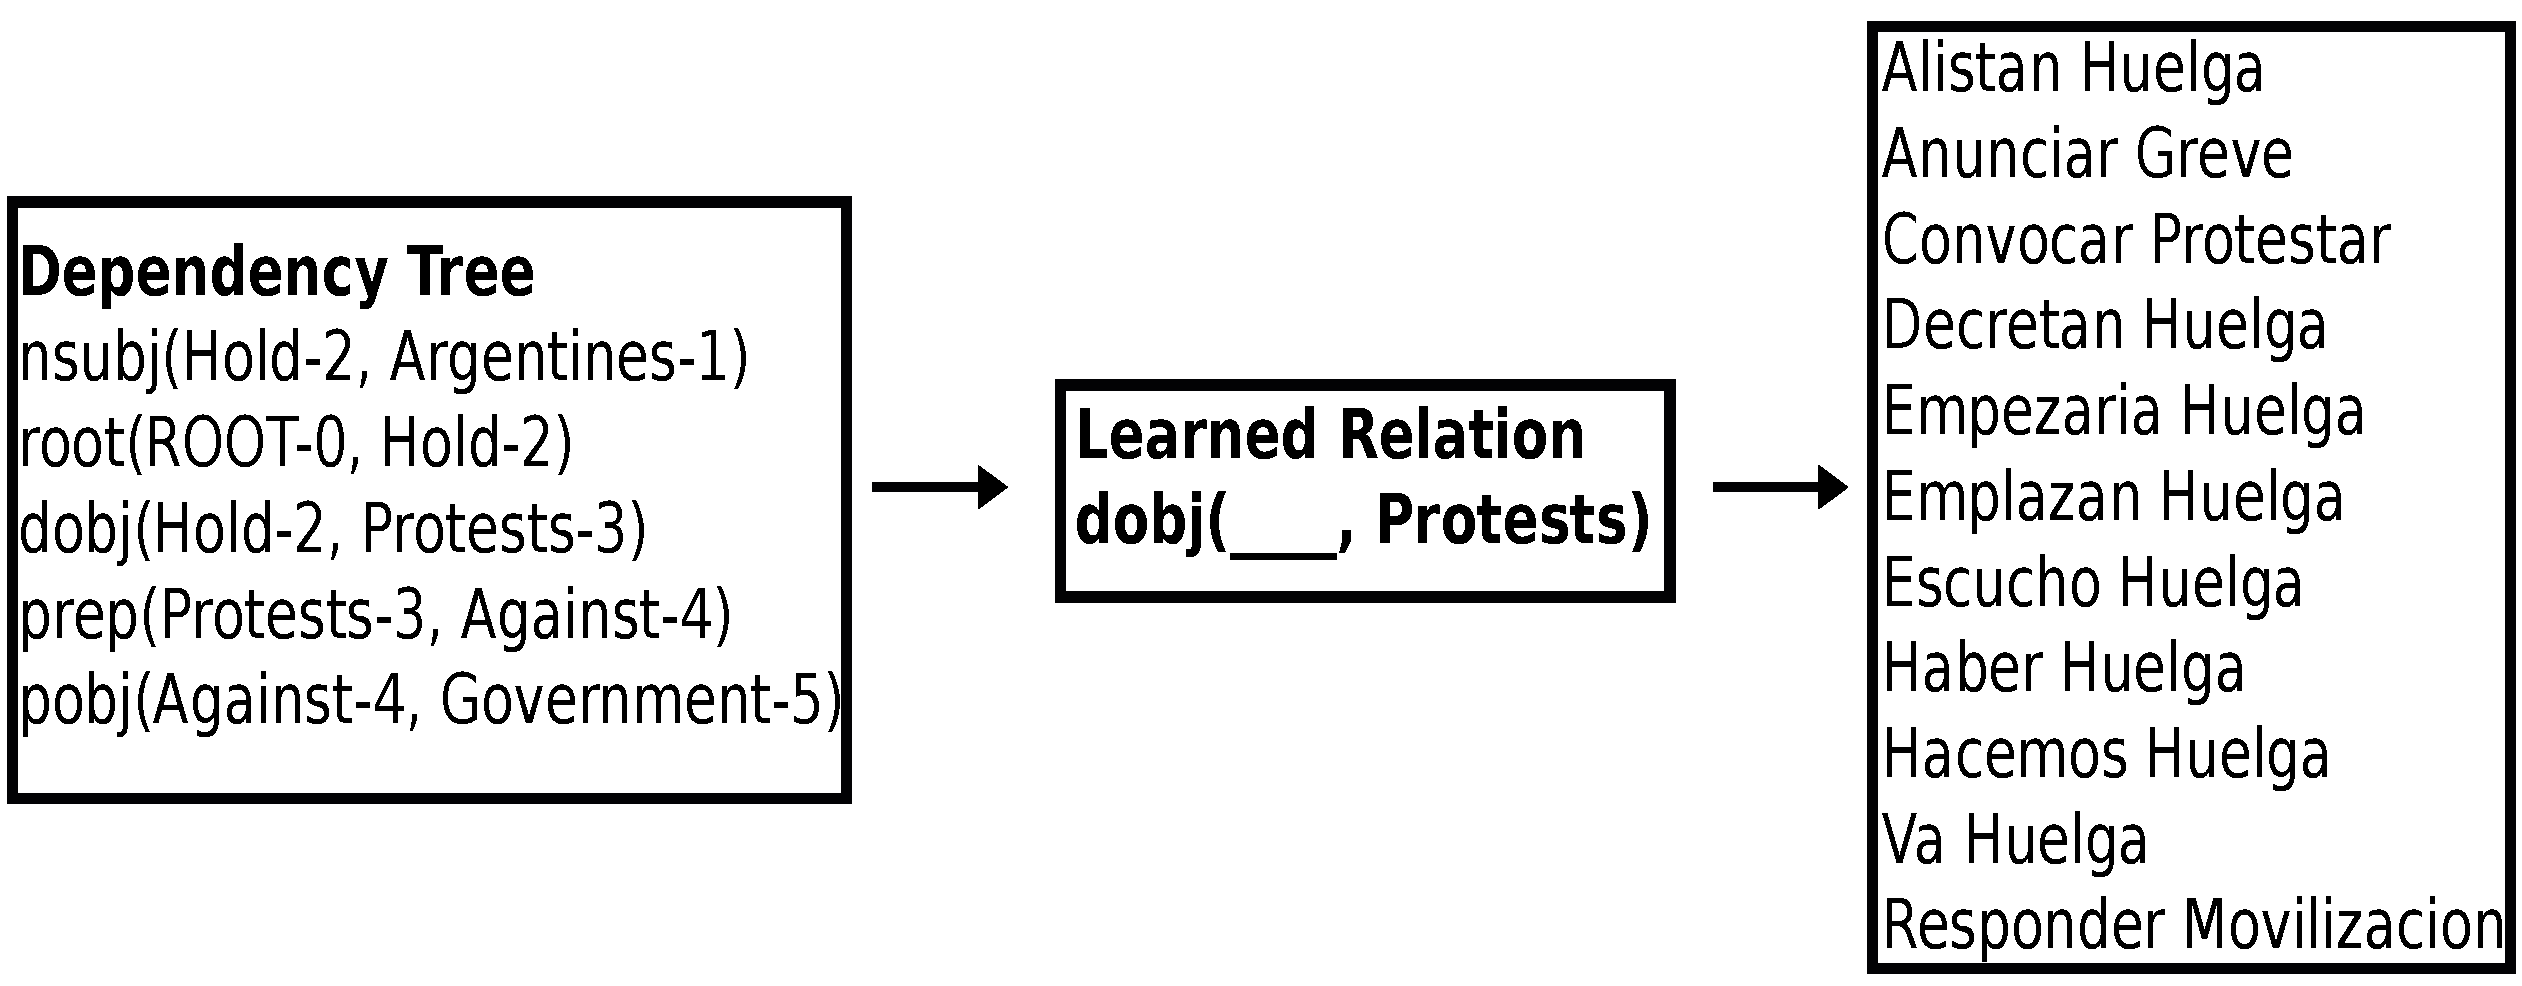
\includegraphics[width=0.5\textwidth]{figures/phraseLearning}
\vspace{-2em}
\caption{An example of phrase learning for detecting planned protests.}
\label{fig:phraselearning}
\end{figure}

\subsection{Geocoding}
\label{subsection:geocoding}
After linguistic preprocessing and suitable phrase filtering,
messages are geocoded with a
specification of the geographical focus of the text---specified as a
city, state, country triple---that indicates the locality that the
text is about. We make use of different geocoding methodologies
for Twitter messages, for Facebook Events pages, and for news articles and blogs.
These are described below.

\vspace{-0.5em}
\subsubsection{Twitter and Facebook}
For tweets, the geo-focus of the message is generated by a fairly
simple set of heuristics involving i)
the most reliable but least
available source, i.e., the geotag (latitude, longitude) of the tweet itself,
ii) Twitter {\it places} metadata, and iii) if the above are not
available, the text fields 
contained in
the user profile (location, description) as well as the tweet text
itself to find mentions of relevant locations.  Additional toponym disambiguiation heuristics are used to
identify the actual referent of the mention.
Similar methods are used to geocode event data extracted from 
Facebook event pages.  

\vspace{-0.5em}
\subsubsection{News and Blogs}
For longer articles such as news articles, the geo-focus of the message
is identified using much more complex methods to extract the protest
location from news articles, we use PSL to build probabilistic models
that infer the intended location of a protest by weighing evidence
coming from the Basis entity extractions and information in the World
Gazeteer. 

The primary rules in the model encode the effect that Basis-extracted
location strings that match to gazatteer aliases are indicators of the
article's location, whether they be country, state, or city aliases.
Each of these implications is conjuncted with a prior for ambiguous,
overloaded aliases that is proportional to the population of the
gazetteer location. For example, if the string ``Los Angeles'' appears
in the article, it could refer to either Los Angeles, California, or Los
\'{A}ngeles in Argentina or Chile. Given no other information, our model
would infer a higher truth value for the article referring to Los
Angeles, California, because it has a much higher population than the
other options. 
\scriptsize
\begin{flalign*}
    ENTITY&(L, location) \softand REFERSTO(L, locID) &\\
                        &\rightarrow FOCUSLOCATION(Article, locID) &
\end{flalign*}

\vspace{-2.5em}
\begin{flalign*}
    ENTITY&(C, location) \softand IsCountry(C) &\\
                        &\rightarrow ArticleCountry(Article, C) &
\end{flalign*}

\vspace{-2.5em}
\begin{flalign*}
    ENTITY&(S, location) \softand IsState(S)&\\
                            &\rightarrow ArticleState(Article, S)&
\end{flalign*}
\normalsize
\noindent
(Note that the above are not deterministic rules; e.g., they do not use
the logical conjunction $\wedge$ but rather the Lukasiewicz t-norm based
relaxation $\softand$. Further, these rules do not fire
deterministically but are instead simultaneously solved for satisfying
assignments as described in the previos section)

The secondary rules, which are given half the weight of the primary
rules, perform the same mapping of extracted strings 
to gazetteer aliases, but for extracted persons and organizations. Strings describing persons and 
organizations often include location clues (e.g., ``mayor of Buenos Aires''), but intuition suggests 
the correlation between the article's location and these clues may be lower than with location strings. 
\scriptsize
\begin{flalign*}
    ENTITY&(O, organization) \softand REFERSTO(O, locID)&\\
                            &\rightarrow FOCUSLOCATION(Article, locID) &
\end{flalign*}

\vspace{-2.5em}
\begin{flalign*}
    ENTITY&(O, organization) \softand IsCountry(O)&\\
        &\rightarrow ArticleCountry(Article, O)&
\end{flalign*}

\vspace{-2.5em}
\begin{flalign*}
    ENTITY&(O, organization) \softand IsState(O)&\\
          &\rightarrow ArticleState(Article, O) &
\end{flalign*}
\normalsize
Finally, the model includes rules and constraints to require consistency between the different levels of geolocation, 
making the model place higher probability on states with its city contained in its state, which is 
contained in its country. As a post-processing step, we enforce this consistency explicitly by using the 
inferred city and its enclosing state and country, but adding these rules into the model makes the 
probabilistic inference prefer consistent predictions, enabling it to combine evidence at all levels.
\scriptsize
\begin{flalign*}
    PSLLOCATION&(Article, locID) \softand Country(locID, C)&\\
               &\rightarrow ArticleCountry(Article, C)&
\end{flalign*}

\vspace{-2.5em}
\begin{flalign*}
    PSLLOCATION&(Article, locID) \softand Admin1(locID, S)&\\
               &\rightarrow ArticleState(Article, S)&
\end{flalign*}
\normalsize

\vspace{-0.8em}
\section{Experiments}
We evaluate our planned protest detection system
using metrics similar to those described in 
Ramakrishnan et al.~\cite{emberskdd}.
Given a set of alerts issued by the system and the GSR comprising actual protest incidents, we aim to identify
a correspondence between the two sets via a bipartite matching.
An alert can be matched to a GSR event only if i) they are both issued for the same country, 
ii) the alert's predicted location and the event's reported location are within 300km of each
other (the distance offset), and iii) the forecasted event date is within a given interval of the true event date (the date offset).
Once these inclusion criteria apply, the quality score (QS) of the match is defined as a combination of the
location score (LS) and date score (DS):
\small
\begin{equation}
    \operatorname{QS}= (LS + DS)*2
\end{equation}
\normalsize
\noindent
where
\small
\begin{equation}
    \operatorname{LS}=1 - \frac{\min(\textrm{distance offset}, 300)}{300}
\end{equation}
and 
\begin{equation}
    \operatorname{DS}=1 - \frac{\min(\textrm{date offset}, \operatorname{INTERVAL})}{\operatorname{INTERVAL}}
\end{equation}
\normalsize
Here, we explore $\operatorname{INTERVAL}$ values from $0$ to $7$.
if an alert (conversely, GSR event) cannot be matched to any GSR event (alert, respectively), these unmatched
alerts (and events) will negatively impact the precision (and recall) of the system. The lead time,
for a matched alert-event pair,
is calculated as the difference between the date on which the forecast was made and the date on which the event
was reported (this should not be confused with the date score, which is the difference between the
predicted event date and the actual event date). Lead time concerns itself with reporting and forecasting, whereas
the date score is concerned with quality or accuracy.
\textcolor{red}{
On average the forecasted event date is within 1.19 days of the true event date and the forecasted location is within 45km of the true location.}

We conduct a series of experiments to evaluate the performance of our system.\\
\begin{figure*}
\centering
\begin{subfigure}{\columnwidth}
  \centering
  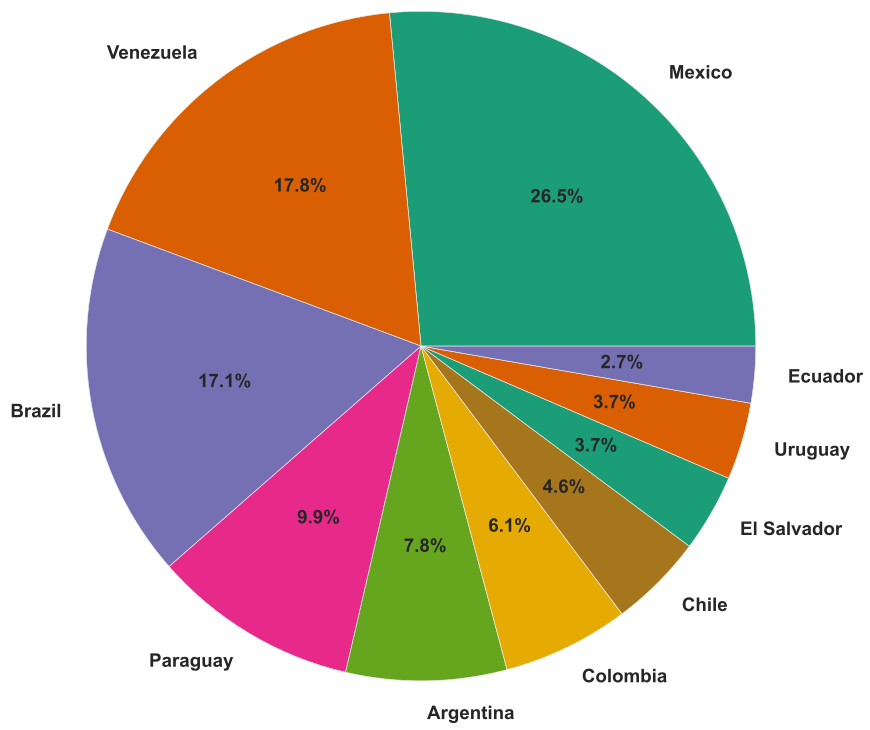
\includegraphics[scale=0.4]{gsr_distribution}
  \vspace{-2em}
  \caption{GSR distribution from 2012-11 to 2014-03.}
  \label{fig:gsrdistribution}
\end{subfigure}%
\begin{subfigure}{\columnwidth}
  \centering
  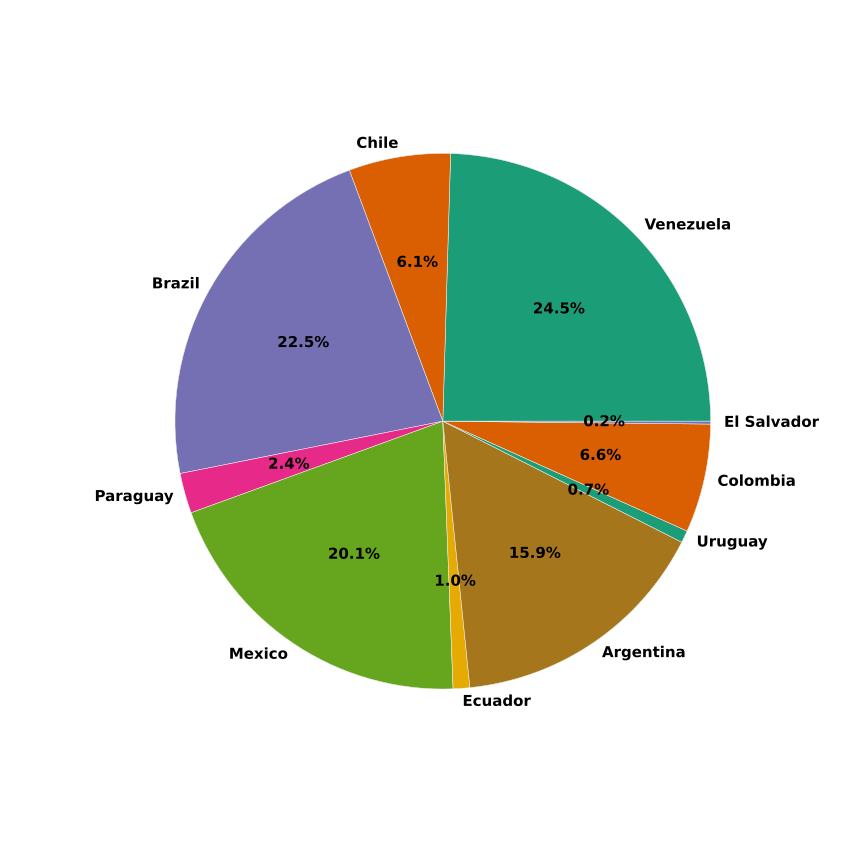
\includegraphics[scale=0.4]{pp_dist}
  \vspace{-2em}
  \caption{Alerts distribution from 2012-11 to 2014-03.}
  \label{fig:ppdistribution}
\end{subfigure}
  \vspace{-.5em}
\caption{Distribution of alerts and GSR events across the countries studied in this paper.}
\label{fig:distribution}
\end{figure*}

\begin{figure*}
\begin{subfigure}{.70\columnwidth}
    \centering
  
\includegraphics[scale=0.2]{monthlyqs}
  \vspace{-0.5em}
  \caption{\scriptsize Quality Score over the months}
  \label{fig:monthlyqs}
\end{subfigure}\hspace{.5pt}
\begin{subfigure}{.70\columnwidth}
    \centering
  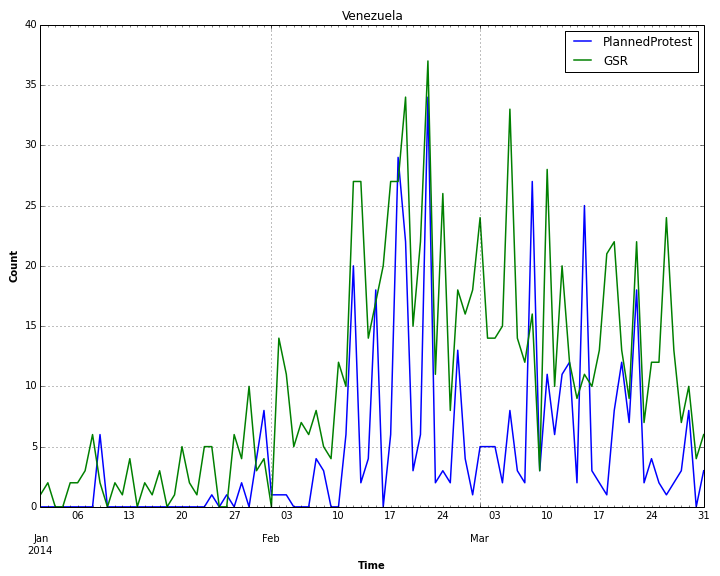
\includegraphics[scale=0.2]{venezuela}
  \vspace{-0.5em}
  \caption{\scriptsize Venezuelan Protests}
  \label{fig:venezuela_feb}
\end{subfigure}\hspace{.5pt}
\begin{subfigure}{.70\columnwidth}
    \centering
  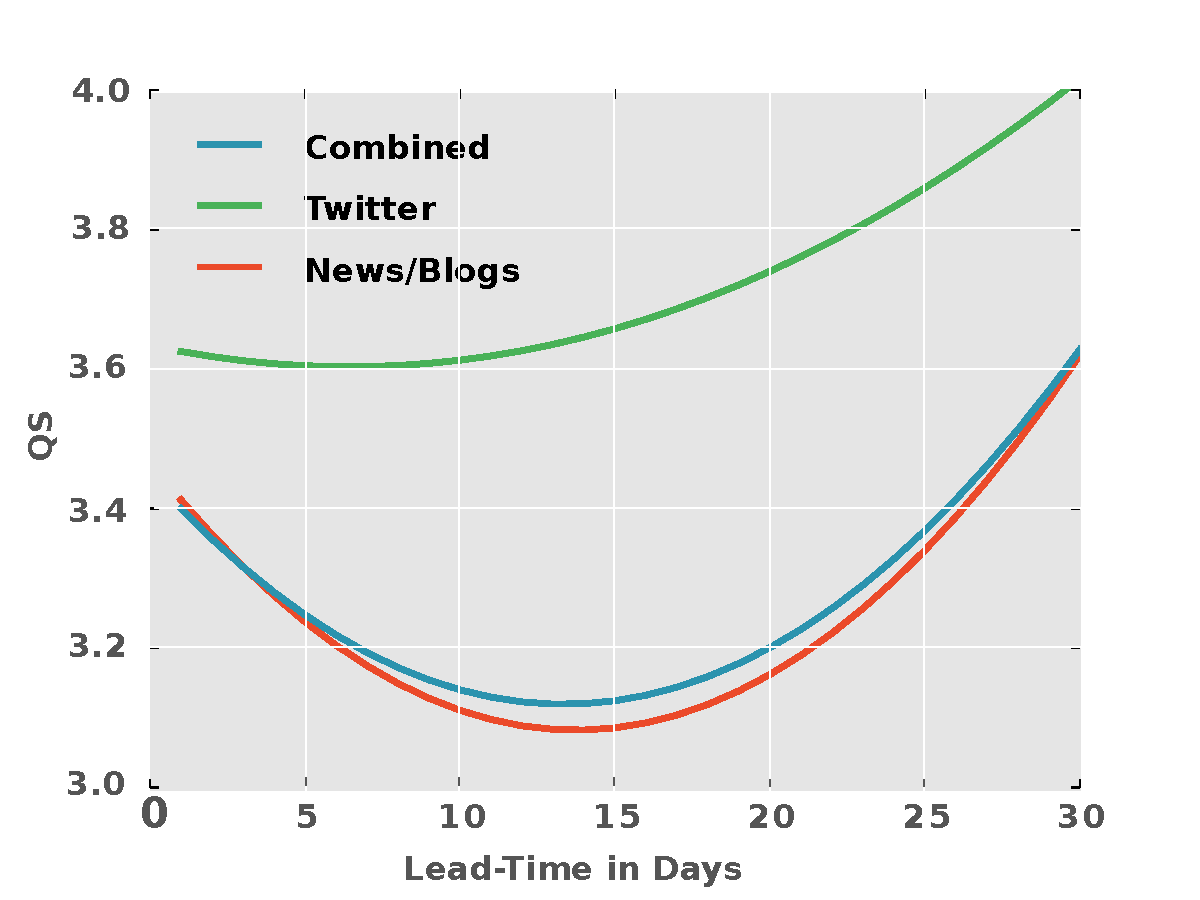
\includegraphics[scale=0.2]{leadTimeVsQS}
  \vspace{-0.5em}
  \caption{\scriptsize Lead-Time vs Quality Score}
  \label{fig:leadTimeVsQS}
\end{subfigure}

\begin{subfigure}{.70\columnwidth}
    \centering
  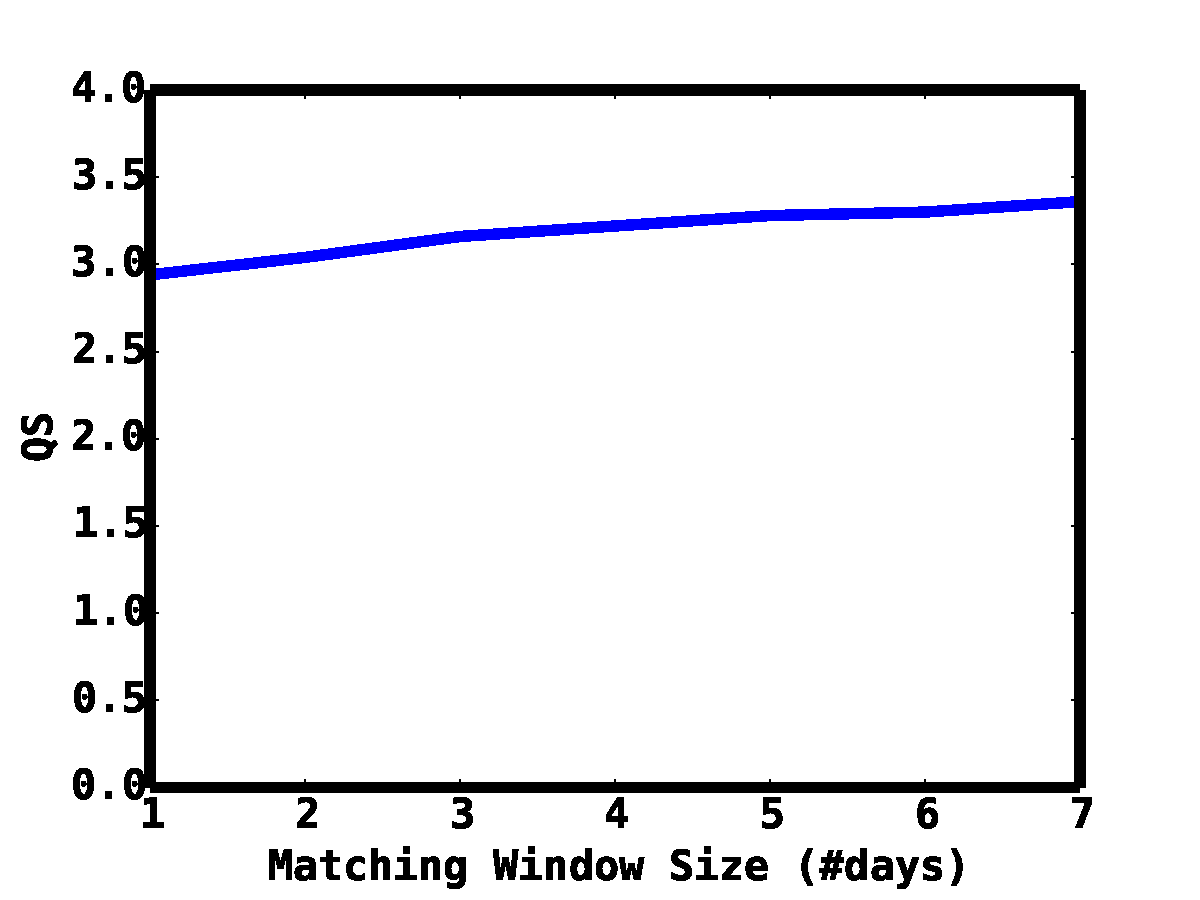
\includegraphics[scale=0.2]{matchingwindow}
  \vspace{-0.5em}
  \caption{\scriptsize QS vs Matching Interval Trade-Off}
  \label{fig:matchinginterval}
\end{subfigure}\hspace{.5pt}
\begin{subfigure}{.70\columnwidth}
    \centering
  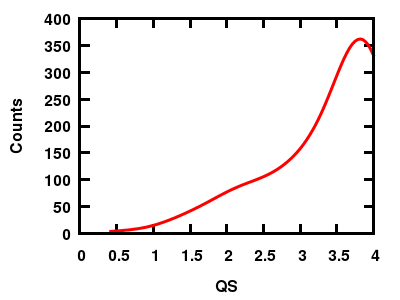
\includegraphics[scale=0.33]{doubleHump}
  \vspace{-1em}
  \caption{\scriptsize Quality Score Distribution}
  \label{fig:doubleHump}
\end{subfigure}\hspace{.5pt}
\begin{subfigure}{.70\columnwidth}
    \centering
  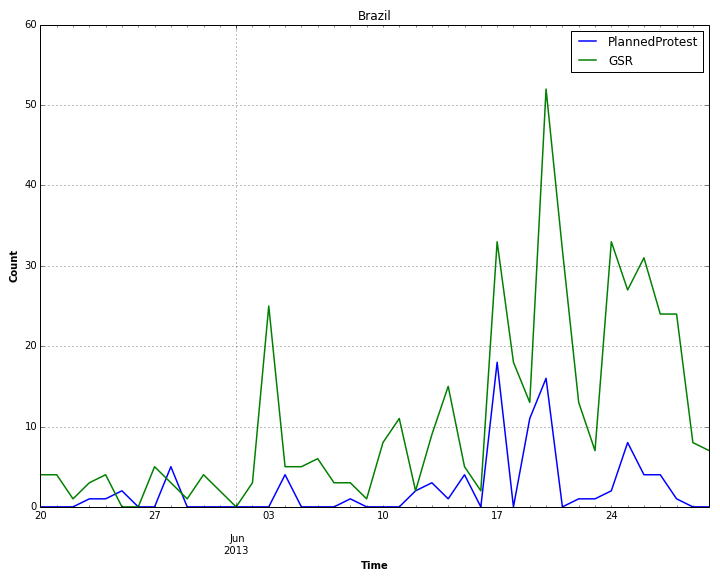
\includegraphics[scale=0.2]{brazil_june}
  \vspace{-0.5em}
  \caption{\scriptsize System Performance during Brazilian Spring}
  \label{fig:brazil_june}
\end{subfigure}\hspace{.5pt}
\caption{Evaluation of planned protest forecasting system}
\end{figure*}

\vspace{-0.8em}
\noindent
{\bf How does the distribution of protests detected by the system compare with the
actual distribution of protests in the GSR?}
Fig.~\ref{fig:distribution} reveals pie charts of both distributions. As shown, Mexico, Brazil, and Venezuela
experience the lion's share of protests in our region of interest, and the protests detected also match these modes
although not the specific percentages. The smaller countries like Ecuador, El Salvador, and Uruguay do experience
protests but which are not as prominently detected as those for other countries; we attribute this to their smaller
social media footprint (relative to countries like Brazil and Venezuela).\\

\begin{table*}
    \small
    \centering
    %\vspace{-2em}
    \caption{\label{tb:sourcewisecomparison} \small Country-wise breakdown of forecasting performance for different data sources.
QS=Quality Score; Pr=Precision; Rec=Recall; LT=Lead Time.
AR=Argentina; BR=Brazil; CL=Chile; CO=Colombia; EC=Ecuador;SV=El Salvador; MX=Mexico; PY=Paraguay; UY=Uruguay; VE=Venezuela. A $-$ indicates that the source did not produce any warnings for that country in the studied period.}
\vspace{-2mm}
    \begin{tabular}{|*{17}{c|}}
        \hline
        & \multicolumn{4}{ |c| }{News/Blogs} & \multicolumn{4}{ |c| }{Twitter} & \multicolumn{4}{ |c| }{Facebook} & \multicolumn{4}{ |c| }{Combined}\\
        \hline
         & QS & Pr. & Rec. &LT & QS & Pr. & Rec. & LT & QS & Pr. & Rec. & LT & QS & Pr. & Rec. & LT\\
        \hline
        AR &3.14&0.32&0.69&3.94&3.52&{\bf0.78}&0.14&3.14&{\bf3.70}&0.50&0.04&3.00&3.02&0.36&{\bf0.80}&{\bf4.50}\\
        BR &3.14&0.48&0.54&{\bf5.85}&-&-&-&-&{\bf3.62}&{\bf0.76}&0.18&2.46&3.28&0.49&{\bf0.65}&5.15\\
        CL &3.06&0.91&0.67&5.40&{\bf3.52}&{\bf1.00}&0.23&4.29&-&-&-&-&3.16&0.83&{\bf0.80}&{\bf5.92}\\
        CO &2.74&0.90&0.56&{\bf7.44}&3.30&{\bf1.00}&0.15&2.43&{\bf4.00}&{\bf1.00}&0.02&2.00&2.88&0.84&{\bf0.65}&6.47\\
        EC &-&-&-&-&{\bf2.32}&{\bf1.00}&{\bf0.06}&{\bf17.00}&-&-&-&-&{\bf2.32}&{\bf0.50}&{\bf0.06}&{\bf17.00}\\
        MX &2.96&0.88&0.25&{\bf3.69}&3.14&{\bf1.00}&0.02&1.43&{\bf3.72}&0.67&0.01&2.00&3.00&0.87&{\bf0.27}&3.51\\
        SV &{\bf3.22}&{\bf1.00}&{\bf0.03}&{\bf1.0}&-&-&-&-&-&-&-&-&{\bf3.22}&{\bf1.0}&{\bf0.03}&{\bf1.0}\\
        PY &3.38&{\bf1.00}&{\bf0.16}&9.11&3.84&{\bf1.00}&0.04&{\bf11.40}&3.96&{\bf1.00}&0.01&2.00&3.60&0.96&{\bf0.20}&9.35\\
        UY &{\bf3.24}&{\bf1.00}&{\bf0.29}&{\bf2.40}&-&-&-&-&-&-&-&-&3.24&{\bf1.00}&{\bf0.29}&3.24\\
        VE &{\bf3.80}&{\bf1.00}&0.36&{\bf3.27}&3.68&0.97&0.33&2.39&-&-&-&-&3.64&0.99&{\bf0.69}&2.88\\
        ALL &3.34&0.69&0.35&{\bf4.57}&3.62&{\bf0.97}&0.15&2.82&3.66&0.74&0.03&2.44&3.36&0.73&{\bf0.51}&4.08\\
        \hline
    \end{tabular}
\end{table*}

\vspace{-0.8em}
\noindent
{\bf Are there country-specific selective superiorities for the different data sources considered here?}
Table~\ref{tb:sourcewisecomparison} presents a breakdown of perfomance, country-wise and source-wise, of 
our approach for a recent month, viz. March 2014.
It is clear that the multiple data sources are necessary to achieve a high recall and that by and large
these sources are providing mutually exclusive alerts. (Note also that some data sources do not produce alerts for specific
countries.) Between Twitter and Facebook, the former is a better
source of alerts for countries like Chile and the latter is a better source for Argentina, Brazil, Colombia, and Mexico.
News and blogs achieve higher recall than social media sources indicating that most plans for protests are announced
in established media. They are also
higher quality sources for alerts in countries like El Salvador, Paraguay, and Uruguay.
Finally, note that news and blogs offer a much higher lead time (4.57 days) 
as compared to that for Facebook (2.44 days) or for Twitter (2.82 days). The quality scores are
further broken down in Table~\ref{tb:modelwisecomparison} into their date and location components.
A longitudunal perspective on quality scores is
given in Fig.~\ref{fig:monthlyqs}. Note that in general Twitter tends to have a higher quality score
as multiple re-tweets of future event mentions is a direct indicator of the popularity of an event as 
well as the intent of people to join an event. 
In contrast, mentions of future events in news do not directly shed any insight into popularity or people's
support for the event's causes.\\

\begin{table*} %[tb!]
\centering
\small
%\vspace{-2em}
\caption{\small Comparing the location and date scores of different sources in specific countries.
AR=Argentina; BR=Brazil; CL=Chile; CO=Colombia; EC=Ecuador;SV=El Salvador; MX=Mexico; PY=Paraguay; UY=Uruguay; VE=Venezuela. A $-$ indicates that the source did not produce any warnings for that country in the studied period.}
\label{tb:modelwisecomparison}
\begin{tabular}{||l|*{17}{c|}}
\hline
Source& & AR & BR & CL & CO & EC & SV & MX & PY & UY & VE & All\\
\hline
\multirow{2}{*}{News/Blogs} &LS &0.82&0.76&0.75&0.60&-&{\bf0.75}&0.66&0.79&{\bf0.79}&{\bf0.95}&0.81\\
                            &DS&0.75&0.81&0.78&0.77&-&{\bf0.86}&0.82&0.90&{\bf0.83}&{\bf0.95}&0.86\\
\hline
\multirow{2}{*}{Facebook} &LS &{\bf1.0}&{\bf0.92}&-&{\bf1.00}&-&-&{\bf0.86}&{\bf0.98}&-&-&{\bf0.93}\\
                          &DS&0.85&{\bf0.89}&-&{\bf1.00}&-&-&{\bf1.00}&{\bf1.00}&-&-&0.90\\
\hline
\multirow{2}{*}{Twitter} &LS &0.88&-&{\bf0.84}&0.81&{\bf0.45}&-&0.71&{\bf0.98}&-&0.91&0.89\\
                         &DS&{\bf0.88}&-&{\bf0.92}&0.84&{\bf0.71}&-&0.86&0.94&-&0.93&{\bf0.92}\\
\hline
\end{tabular}
\vspace{-4mm}
\end{table*}

\vspace{-0.8em}
\noindent
{\bf How did our system fare in detecting key country-wide protests?}
The recent Venezuelan protests against President Nicolas Maduro and the Brazilian Protests during June 2013 against bus fare hike were two significant protests during our period of evaluation. Fig.~\ref{fig:venezuela_feb} and
Fig.~\ref{fig:brazil_june} describe our performance under these two situations illustrating the count
of protests detected against the GSR. Notice that our system was able to 
identify the Venezuelan protests much better than the Brazilian protests. This is because there was a significant amount
of spontaineity to the Brazilian protests; they arose as discontent about bus fare increases but later morphed into a broader
set of protests against government and most of these subsequent protests were not planned.\\

\vspace{-0.8em}
\noindent
{\bf What is the tradeoff between lead time and quality?}
Fig.~\ref{fig:leadTimeVsQS} shows that the QS of the planned protest model decreases (as expected) with lead time, initially, but
later rises again. The higher quality scores toward the right of Fig.~\ref{fig:leadTimeVsQS} are primarily due to
Facebook event pages.\\

\vspace{-0.8em}
\noindent
{\bf How does the method perform under stringent matching criteria?}
Fig.~\ref{fig:matchinginterval} shows the perfomance of the model when the matching window is varied from 7 to 1 in steps. 
We can see that the performance degrades quite gracefully even under the strict matching interval of a 1-day difference.\\

\vspace{-0.8em}
\noindent
{\bf What is the distribution of quality scores?}
The clear mode toward the right side of the Fig.~\ref{fig:doubleHump} signifies that a majority of the planned 
protest alerts are of high quality. Further, the quality score distribution is unimodal suggesting that the careful
reasoning of locations and date normalization are crucial to achieving high quality.

\vspace{-0.8em}
\section{Development and Maintenance}
The core algorithms behind the
planned protest detector were implemented in Python. The PSL geocoder was
implemented in Java. The Basis Rosette Linguistic Platform is the key
external library utilized. The development process took 3 months (June
2012 to Aug 2012) and was
primarily led by the first author with contributions from the other authors.
After two months of testing (Sep 2012 and Oct 2012), the system was deployed
in Nov 2012. Since there is not an explicit training
phase, the system has required minimal re-engineering over time. Key changes
made to the system over time was to increase the sources used for data ingest
and supporting the inclusion of additional phrases. Agile software
engineering methods were used for project management.

\vspace{-0.8em}
{\small
\section{Discussion}
We have described an approach to forecasting protests by detecting mentions of future events in news and social
media. The two twin issues of i) resolving the date and ii) resolving the location have been addressed satisfactorily
to realize an effective protest forecasting system. As different forms of communication media gain usage, systems
like ours will be crucial to understanding the concerns of citizenry.As stated in the introduction, there are many legitimate applications of a protest forecasting system such as ours; our goal is to provide advance warnings of protest occurrences to all relevant stakeholders.

Our future work is aimed at three aspects. First, to address situations such as nationwide protests and systems of protests,
we must generalize our system from generating protests at a single article level to digesting groups of articles. This will
require more sophisticated reasoning using PSL programs. 
Second, we would like to generalize our approach that currently
does detection of overt plans for protest to not-so-explicitly stated expressions of discontent. 
Finally, we plan to consider other population-level events of interest than just civil unrest, e.g., domestic political crises,
and design detectors to recognize the imminence of such events.

\vspace{-0.8em}
\section*{Acknowledgments}
Supported by the Intelligence Advanced Research Projects Activity (IARPA) via
DoI/NBC contract number D12PC000337, the US Government is authorized to reproduce and distribute reprints of
this work for Governmental purposes notwithstanding any copyright annotation thereon.
Disclaimer: The views and conclusions contained herein are those of the authors and should not be interpreted as necessarily representing the official policies or endorsements, either expressed or implied, of IARPA, DoI/NBC, or the US Government.
}\vspace{-1em}
\small
\bibliographystyle{aaai}
\bibliography{references}
\end{document}
